\begin{figure}
\caption{Forecast Errors}\label{fg2:fe}\vspace*{1pc}\hspace*{-0.28in}
\begin{tabular}{cccc}
\multicolumn{4}{c}{Case 1: Rational Expectations} \\ 
Consumption & Investment & Inflation & Fed Funds \\
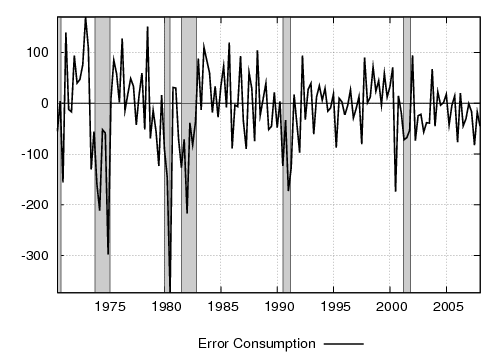
\includegraphics[scale=0.22]{results_re/consumption_err.png} & 
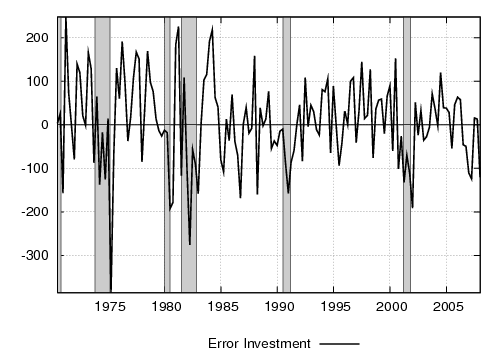
\includegraphics[scale=0.22]{results_re/investment_err.png} & 
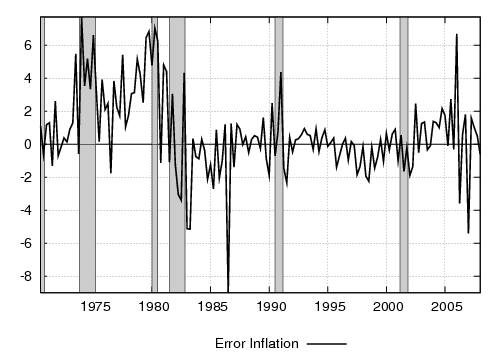
\includegraphics[scale=0.22]{results_re/inflation_err.png} & 
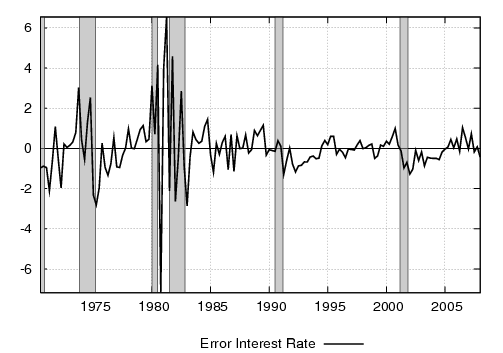
\includegraphics[scale=0.22]{results_re/fedfunds_err.png} \\ \\ 
 
\multicolumn{4}{c}{Case 2: Learing with RE Initial Conditions} \\ 
Consumption (0.9467) & Investment (0.8525) & Inflation (0.9235) & Fed Funds (0.9512) \\
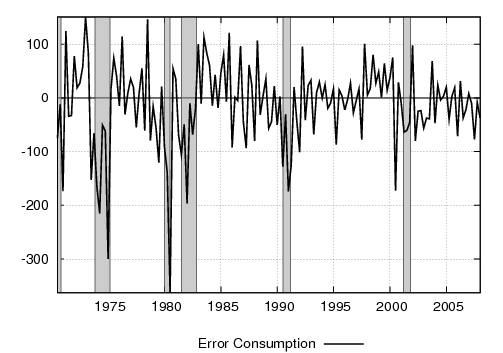
\includegraphics[scale=0.22]{results_reallinit/consumption_err.png} & 
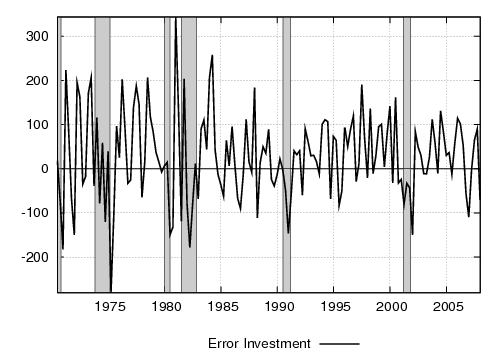
\includegraphics[scale=0.22]{results_reallinit/investment_err.png} & 
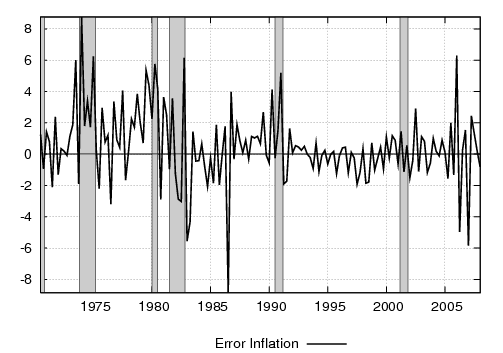
\includegraphics[scale=0.22]{results_reallinit/inflation_err.png} & 
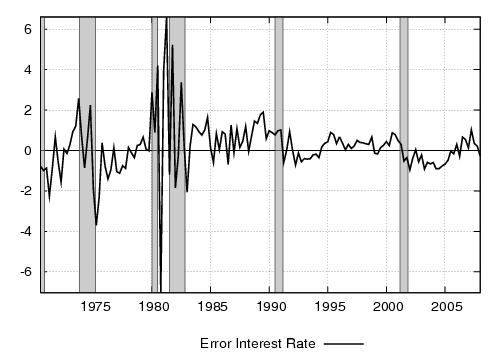
\includegraphics[scale=0.22]{results_reallinit/fedfunds_err.png} \\ \\ 
 
\multicolumn{4}{c}{Case 3: Learing with RE Initial Conditions, Shocks Unobservable} \\ 
Consumption (0.9922) & Investment (0.8598) & Inflation (0.6517) & Fed Funds (0.9474) \\
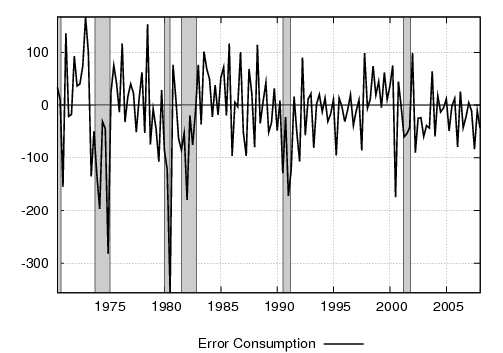
\includegraphics[scale=0.22]{results_reinit/consumption_err.png} & 
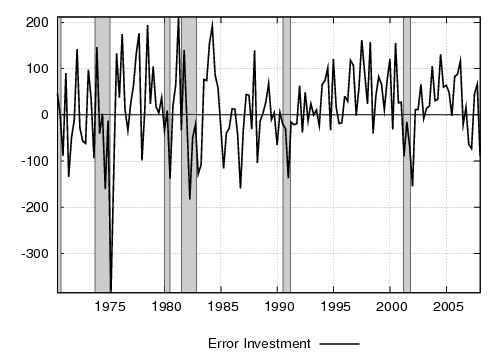
\includegraphics[scale=0.22]{results_reinit/investment_err.png} & 
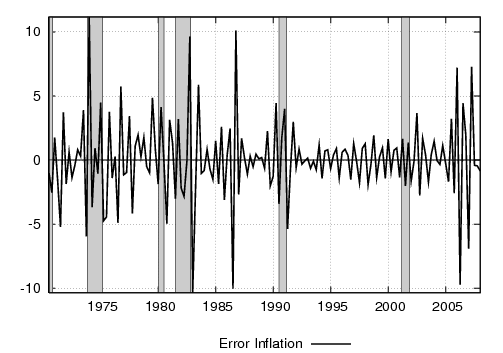
\includegraphics[scale=0.22]{results_reinit/inflation_err.png} & 
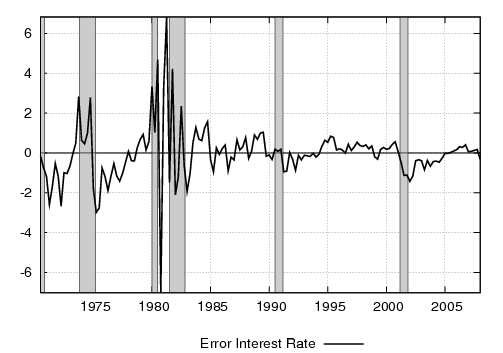
\includegraphics[scale=0.22]{results_reinit/fedfunds_err.png} \\ \\ 
 
\multicolumn{4}{c}{Case 4: Learning with Unobservable Shocks and Pre-Sample Initial Conditions} \\ 
Consumption (0.7003) & Investment (0.4776) & Inflation (0.6457) & Fed Funds (0.6882) \\
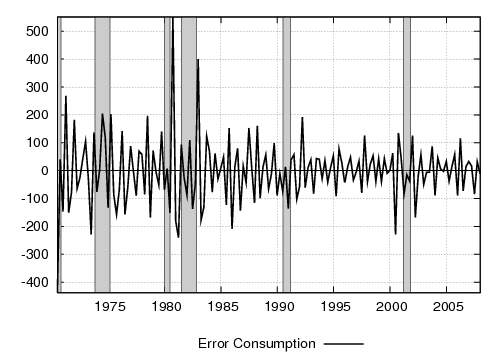
\includegraphics[scale=0.22]{results_wlsinit/consumption_err.png} & 
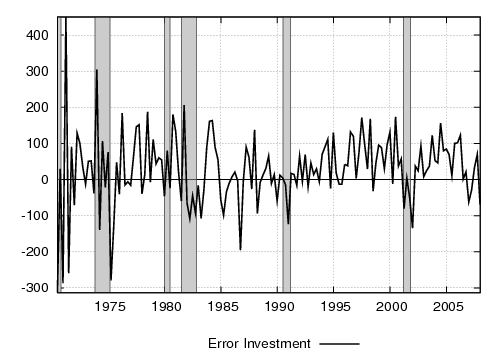
\includegraphics[scale=0.22]{results_wlsinit/investment_err.png} & 
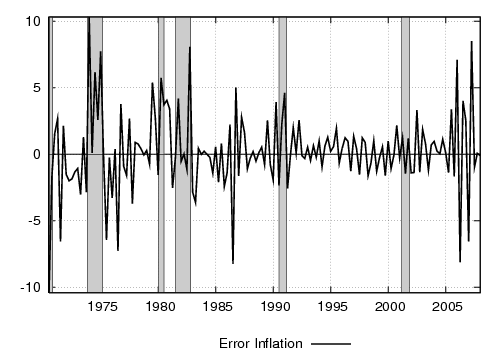
\includegraphics[scale=0.22]{results_wlsinit/inflation_err.png} & 
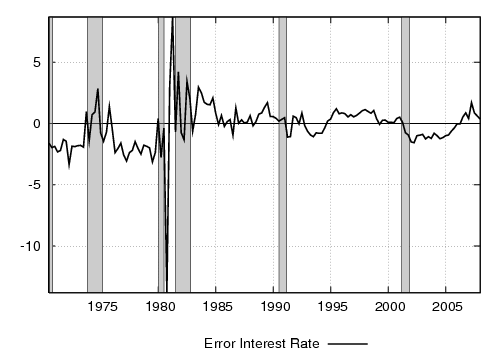
\includegraphics[scale=0.22]{results_wlsinit/fedfunds_err.png} \\ \\ 
 
\end{tabular}
\end{figure}
